\section{Detectors for Collider Physics}
\label{sec:detectors}

In this section we review the basic concepts that drive the design of the LHC detectors, including ATLAS.

\subsection{Identification of Particles}

The ability to accurately identify particles and reconstruct their energy is what drives the design of detectors for high energy physics. In a detector, different sub-systems are able to capture different types of particle interaction, and the combination of the information collected by each of them allows to identify particles (or at least assign them to families, such as neutral or charged hadrons). A typical schema of the subdetectors sequence is shown in Fig. \ref{fig:detector:interaction}. The innermost layer, closer to the interaction point, is the \textit{tracking system}, dedicated to the measurement of the signed change and momentum of charged particles. The following layers are the electromagnetic and hadronic \textit{calorimeters}, that measure the energy of particles with electromagnetic and hadronic interactions respectively. The outermost layer is dedicated to the \textit{muon system}: because of their large mass (about 200 times more than electrons) muons do not produce electromagnetic showers and are therefore easy to identify as they are the only particles that reach the external part of the detector.

\begin{figure}[ht]
\centering
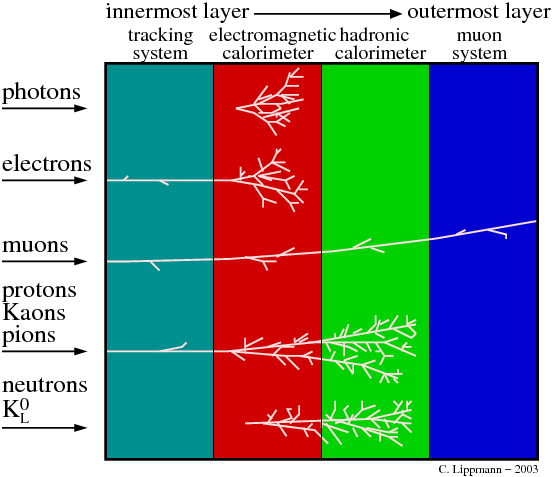
\includegraphics[width=0.6\textwidth]{figures/detector/particles_in_detector}
\caption{Components of a typical detector for physics at colliders. Different particles are identified by the distinctive signatures in the subdetectors. Figure from Ref. \cite{Lippmann:2011bb}.}
\label{fig:detector:interaction}
\end{figure}


\subsection{Tracking and Spectrometry}
\label{sec:dec:tracking}
A tracking device measures the traces left by charged particles passing through it. To allow the determination of the momentum and the charge of a particle, a tracking device needs to be accompanied by a magnetic field (and in this case we speak of a \textit{magnetic spectrometer}): once the magnetic field is known, the measure of the radius of curvature of the particle is equivalent to a measure of its momentum, according to Eq. \ref{eq:cern:p03br}. In a typical particle detector as the one in the schema in Fig. \ref{fig:detector:interaction}, both the inner tracking system and the muon system are magnetic spectrometers.

The relative uncertainty on the momentum is given by:
\begin{equation}
\frac{\sigma_p}{p} = \sqrt{ \left(a p \right)^2 + b^2} \; .
\label{eq:tracking:reso}
\end{equation}

The first term, whose relative importance increases for high-momentum particles, derives from the angular measurement resolution. Typical values for $a$ are between 0.01\% and 1\%. The constant term in Eq. \ref{eq:tracking:reso} accounts for the impact of multiple Coulomb scattering, that broadens the distribution of the transverse momentum perpendicular to the direction of motion. This terms is important only at low energies, while is negligible for high-energy particles.

There are three main configurations of magnetic fields for momentum spectrometers:
\begin{itemize}
\item A \textit{dipole} field leads to a rectangular symmetry; if we think of a circular collider with a coordinate system where $z$ is the direction along the beam trajectory and ($x$,$y$) define a Cartesian system in the transverse plane, a dipole  field in the $x$ direction will cause a deflection in the ($y,z$) plane. This is the configuration adopted by forward spectrometers like LHCb, where the tracking devices are arranged in sequence in the z direction. As an example, the integral of the LHCb dipole field over the detector length is 4 Tm.
\item A \textit{solenoidal} field leads to a cylindrical symmetry and, if the field lines are along the $z$ direction, the deflection is in the ($x,y$) plane. This is the typical configuration of the spectrometers in the central barrel, where the detectors are arranged in cylindrical layers. The CMS solenoid field is 4 T, while the ATLAS one is 2 T. 
\item A \textit{toroidal} field leads to an azymuthal symmetry: the direction of the field lines is a circle in the transverse plane, and a deflection is in the ($r,z$) plane. This configuration is adopted by the ATLAS muon spectrometer, with a magnetic field of 0.5 T. As in the case of the solenoidal field, the detectors are arranged in cylindrical shells.
\end{itemize}

The track left by the charge particles curving because of the magnetic field is reconstructed by the tracking detectors. The two most common categories of tracking devices are gas and silicon detectors, described in the next two sections.

\subsubsection{Gas Detectors}

In gas detectors, the passage of a charge particle ionizes the atoms and creates electron-ion pairs. Once the electron and the ion are created, they can be separated (thus creating a current) by applying an electric field. This induces signal on an electrode added to the material, read through a readout system. The basic principle of most of gas detectors relies on a tube with a wire in the center, which is an anode with an high electric field. When the particle crosses the gas, the electrons drift toward the anode and can be collected. Without electric field, the electron and ion move in the system by thermal diffusion. The effect of an electric field is to make the electron and ion to move in opposite directions, allowing us to measure them. Since not many electrons are produced in gas, they need to be amplified. Inside the tube, decreases with the inverse of the distance from the anode wire. When the electrons reach a distance of a few micrometers from the wire, the electric field is very large and the electrons gain more energy than the ionization energy; this leads to secondary ionization and an exponential growth of the electron-ion pairs (\textit{avalanche effect}). 

Several types of gas detectors with different characteristics have been developed. In \textit{single-wire proportional chambers}, like the one used in the outer tracker of the LHCb experiment, several counters are combined next to each other, to allow the measurement of the particle position. In \textit{multi-wire proportional chambers} \cite{CHARPAK1968262} several wires in two perpendicular directions are contained in the same box filled with gas. \textit{Drift chambers} are a further evolution of wire chambers, where the position of the particle is computed by measuring the time took by the secondary ionization to reach the anode. \textit{Time projection chambers} (TPC) are a different type of gas detector, used for example in ALICE, constituted by a large area filled only with gas, without wires, with detectors and readout structure only at the end plates. Between the plates a strong electric field causes the electron-ion pairs to drift, until they reach the plates where a combined measurement of position and time of arrival allows to reconstruct the three-dimensional trajectory of the particles (that can be curved if a magnetic field is added). \textit{Micro-strips chambers} \cite{OED1988351} are more modern, very condensed and thin gas detectors. Instead of being generated by a wire, the electric field comes from small metal deposits on a high-resistivity substrate.   

In general the main problems of gas detectors are the spatial extension and the long drift time, that make them suitable for the outer part of the LHC detectors, in particular muon spectrometers.

\subsubsection{Solid-state Detectors}

Silicon detectors are the main type of solid-state detectors, and are currently the most used for the inner tracking, where you need higher precision and low occupancy \cite{Hartmann:2009zza}. These detectors detectors are also based on the ionization of the material but in this case, since the structure is a crystal, we talk about electrons and \textit{electron holes}. 

The underlying principle is based on the \textit{band model} of solids.

\begin{figure}[ht]
\centering
\subfigure{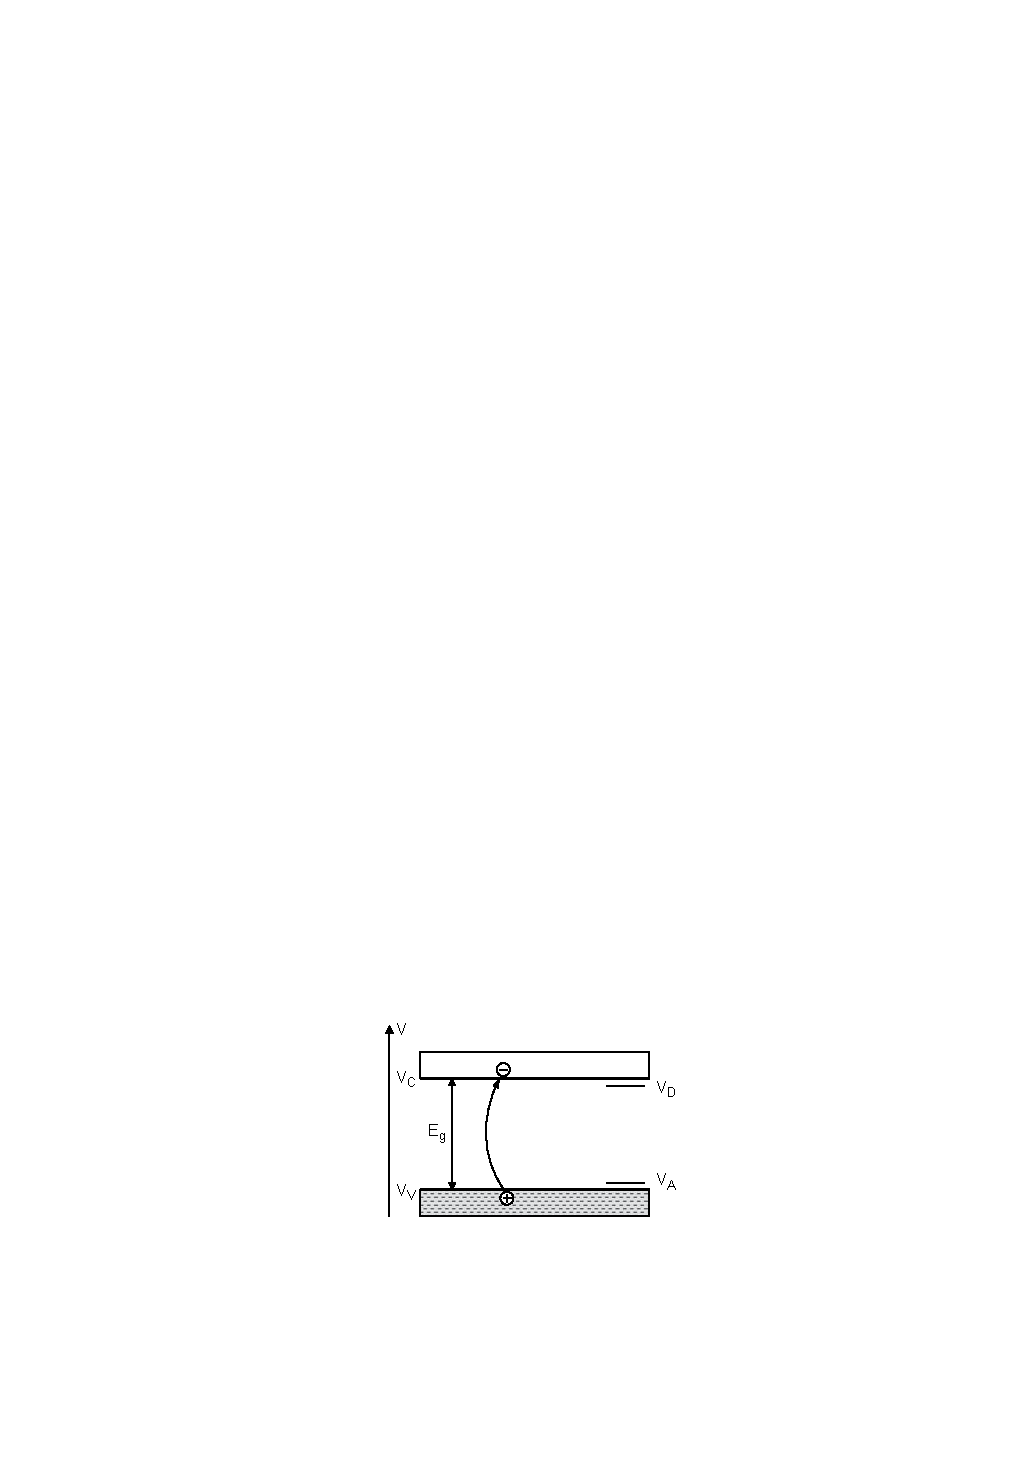
\includegraphics[width=0.45\textwidth]{figures/detector/band_structure}}
\caption{Figure frmo Ref. \cite{grupen_shwartz_2008}.}
\label{fig:det:band}
\end{figure}




The density of silicon is about one thousand higher than the density of gases like argon, and also need a much lower energy to be ionized (3.6 eV for silicon, while it is about 250 times higher for argon). This leads to a much higher number of electron-holes pairs than the number of electron-ion pairs in gas detectors, so the signal needs very little amplification, and the size of the detector itself can be smaller. 

\begin{figure}[ht]
\centering
\subfigure[]{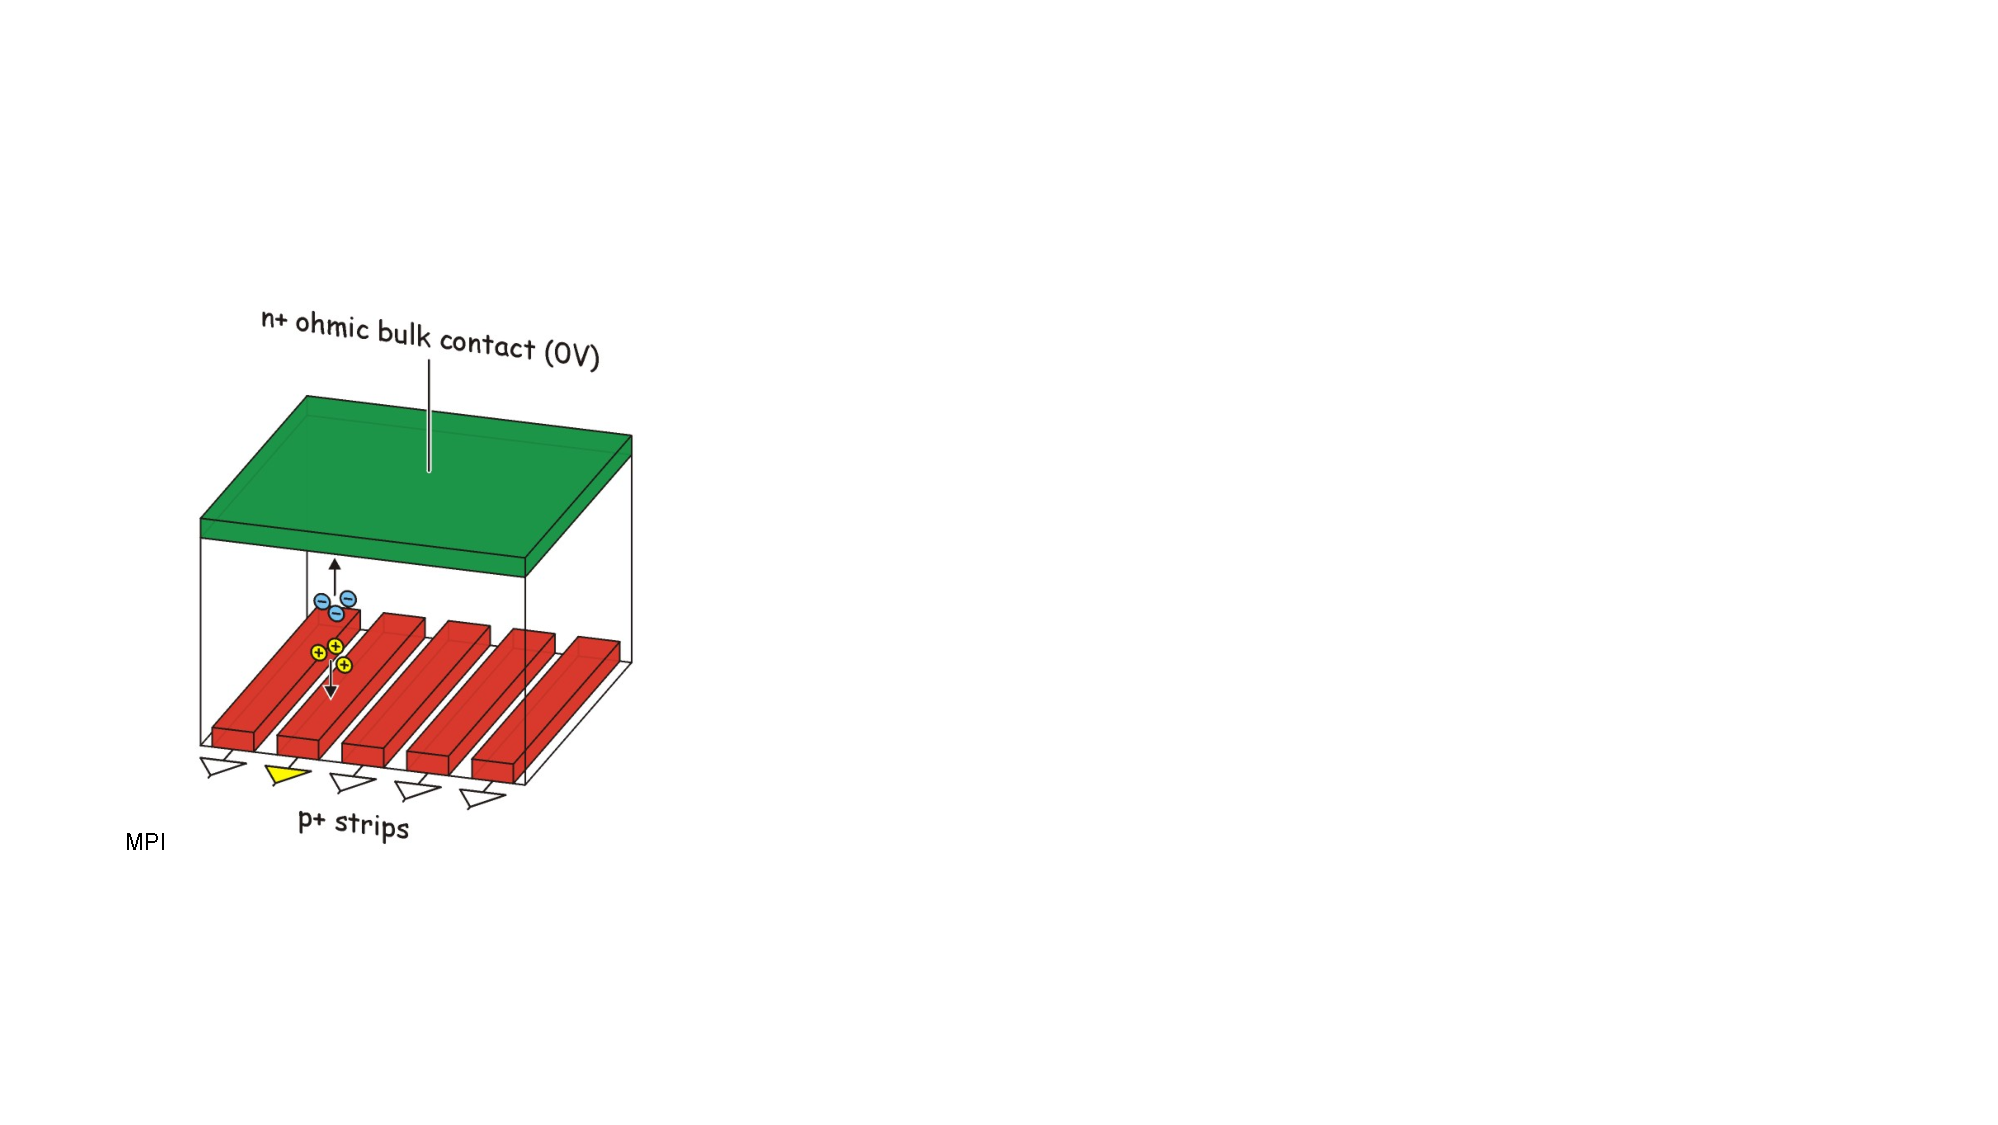
\includegraphics[width=0.32\textwidth]{figures/detector/single-sided-AC-coupled-silicon-strip.pdf}}
\subfigure[]{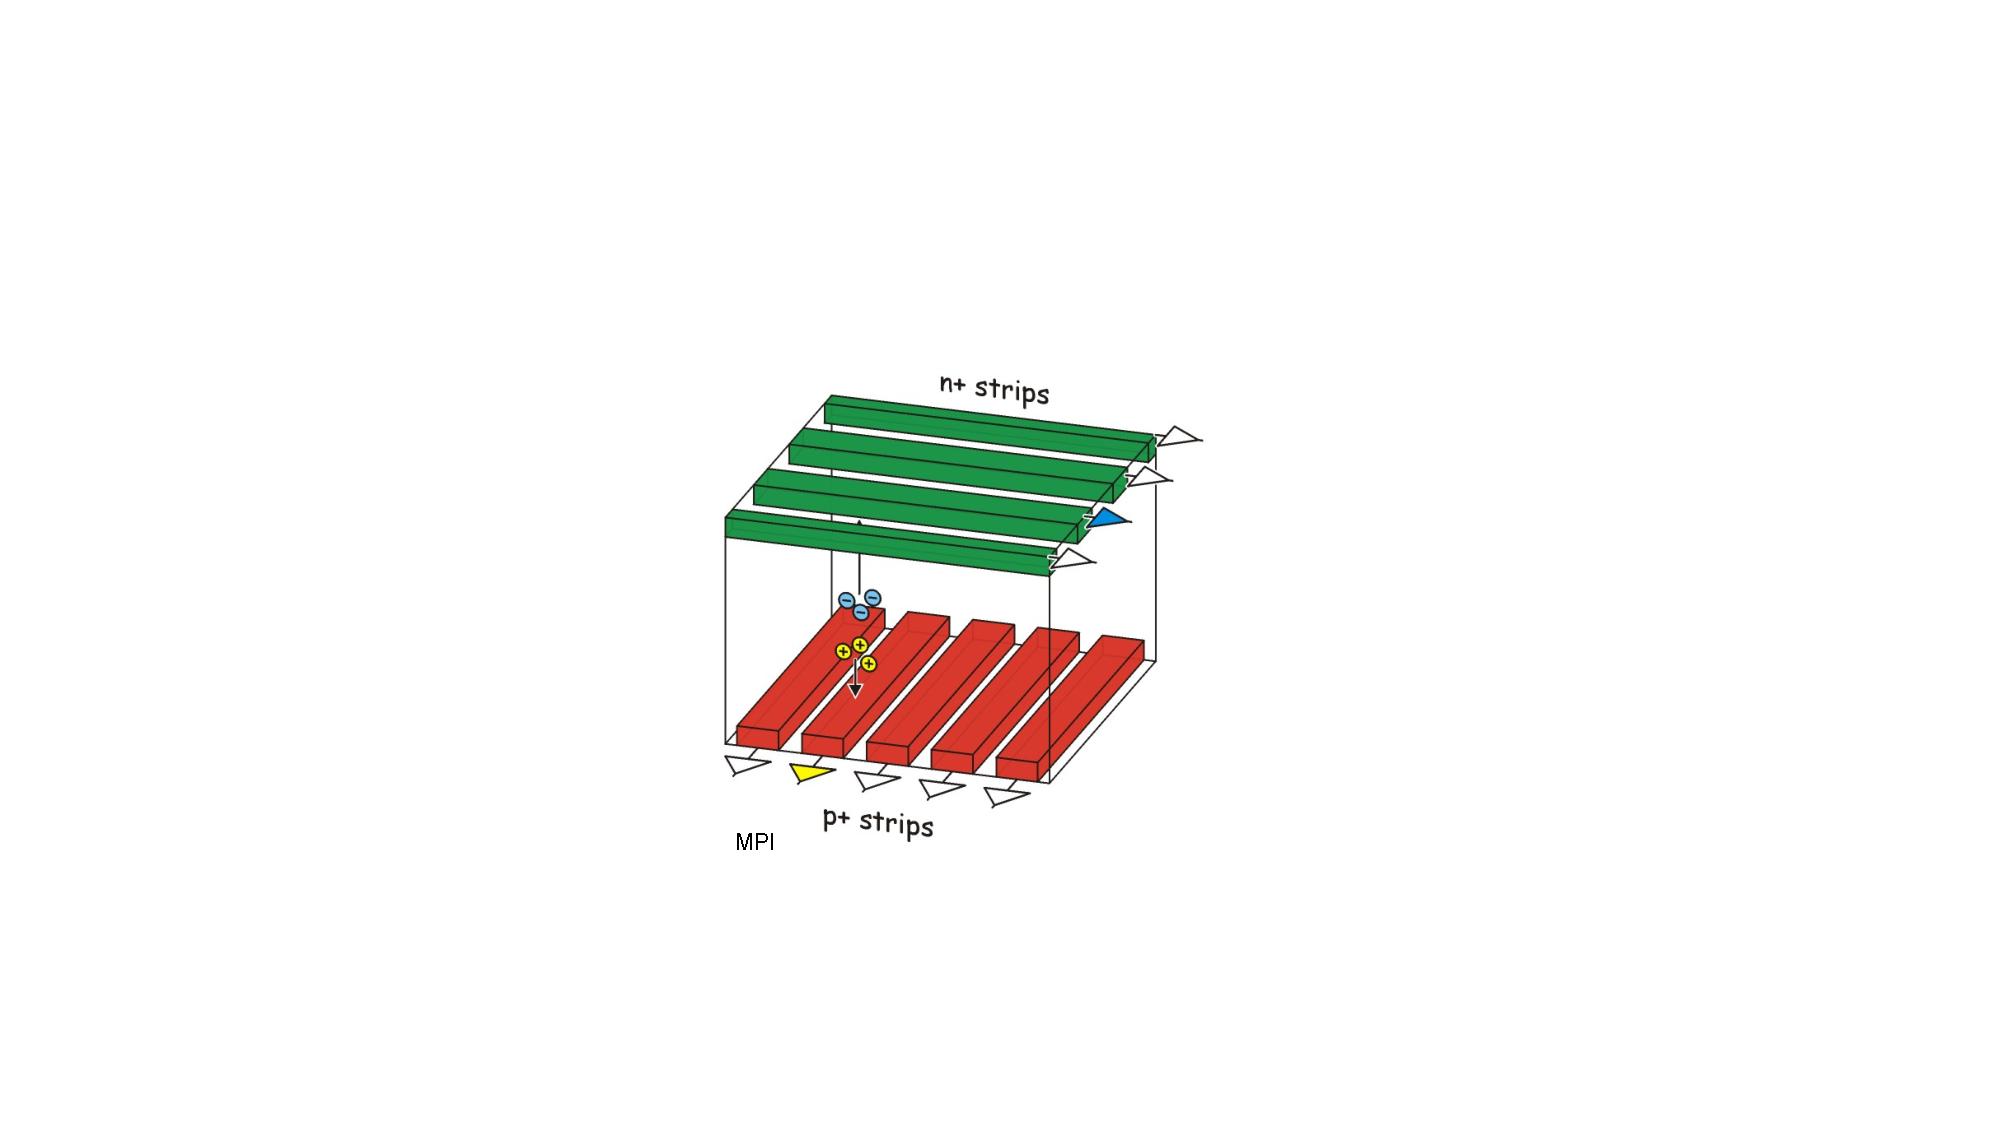
\includegraphics[width=0.32\textwidth]{figures/detector/double-sided-silicon-strip.pdf}}
\subfigure[]{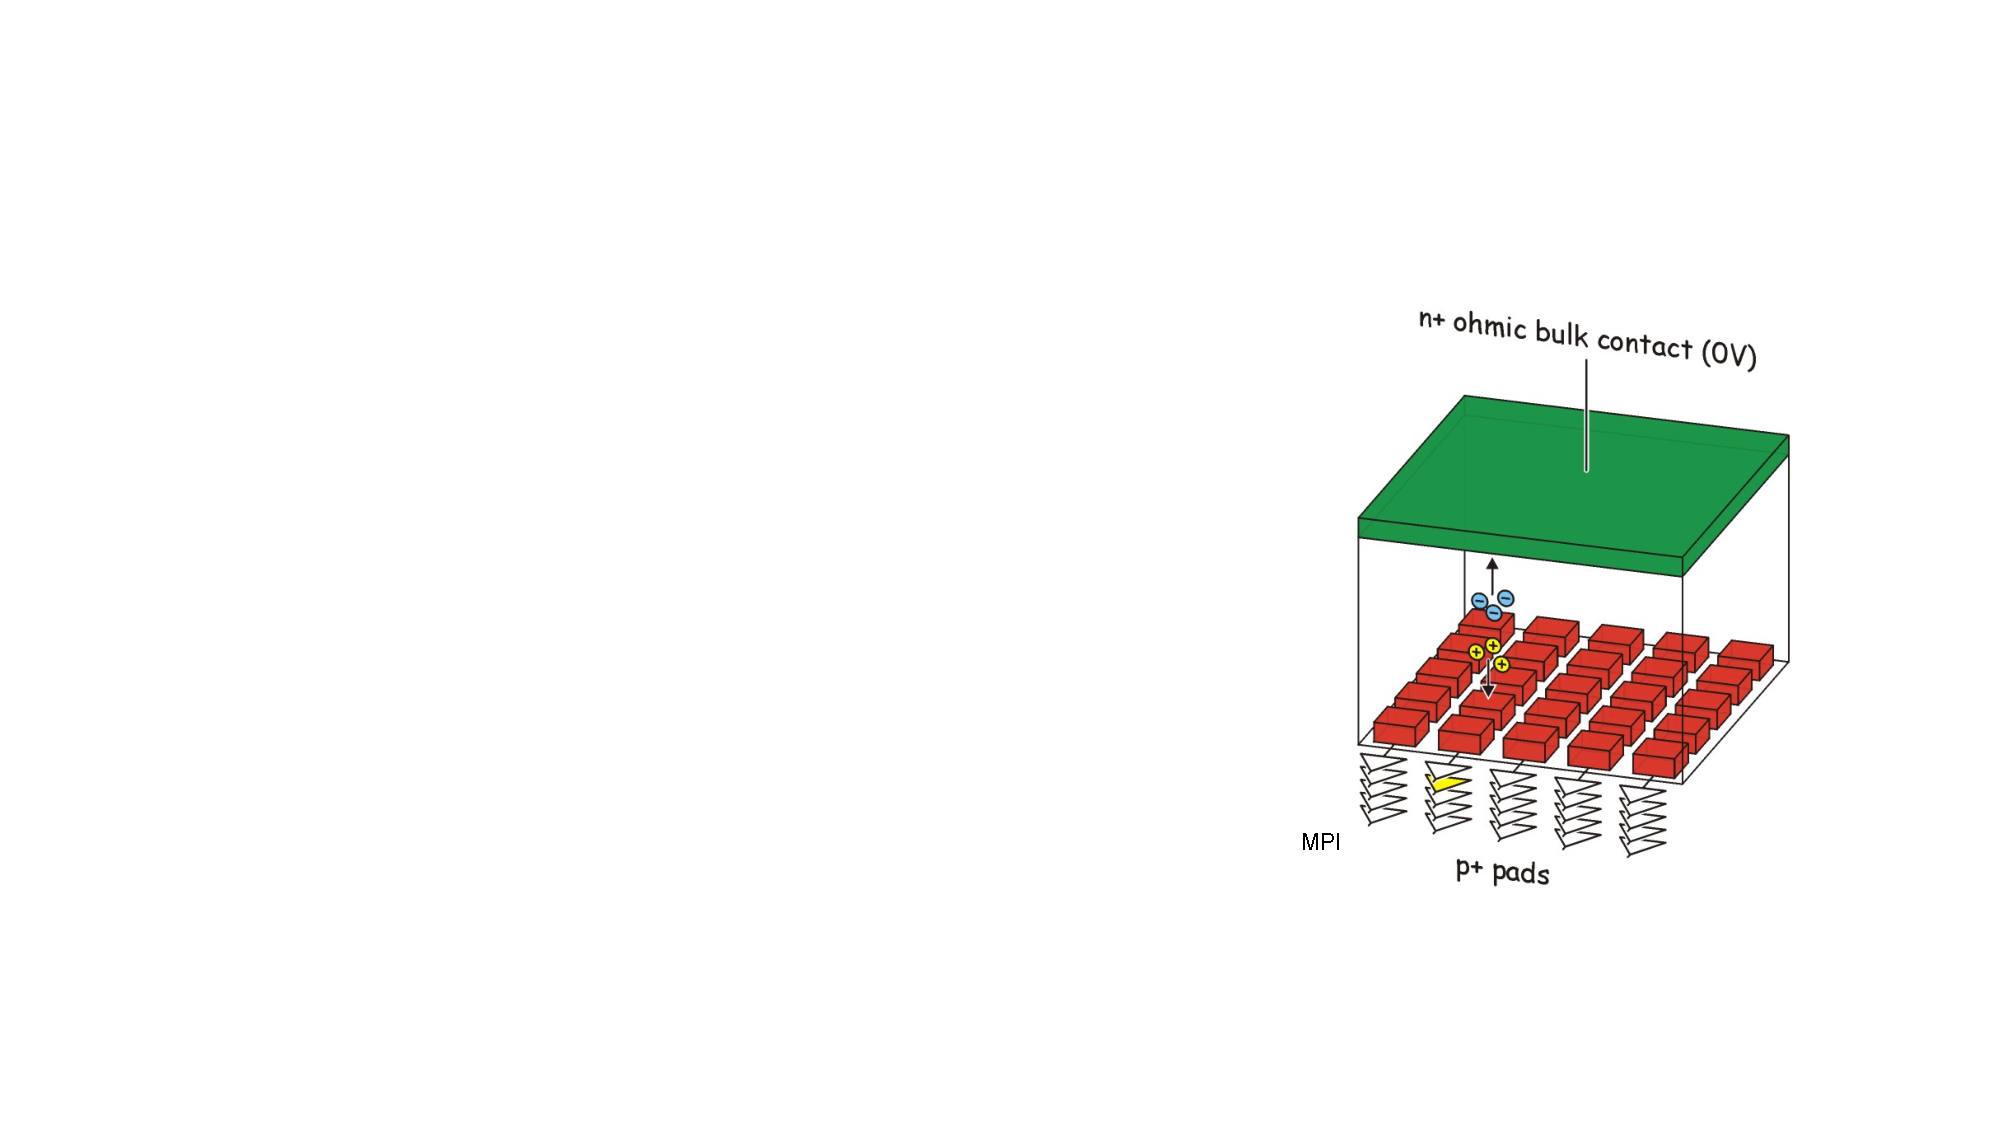
\includegraphics[width=0.32\textwidth]{figures/detector/pixel-schema.pdf}}
\caption{Schematic view of a single-sided strip sensor (a), double-sided strip sensor (b) and pixel module (c). }
\label{fig:det:shower_elec}
\end{figure}

\subsection{Calorimetry}
\label{sec:dec:calo}

Calorimeters can measure the energy of both charged and neutral particles through a destructive measurement: the energy of the particles is deposited in the detector material and transformed into a measurable quantity. Because of their sensitivity to a wide variety of particles, good energy resolution and relatively small size, they are very attractive devices for accelerator physics experiments \cite{RevModPhys.75.1243} \cite{Wigmans:2000vf}.

When the incident particle interacts with the material of the calorimeter it develops a cascade of particles (\textit{shower}), with different characteristics for electromagnetic and hadronic interactions, described in the next two sections. Different types of calorimeters are necessary to capture the two typologies. The energy of the shower is decreased by the interactions happening in the \textit{absorber} material, while the \textit{active} material provides the conversion of the energy in a charge or light signal. In \textit{sampling calorimeters} layers of absorber and active material are alternated in sequence, while in \textit{homogeneous calorimeters} a single material carries out both functions.


\subsubsection{Electromagnetic Calorimeters}

The type of interaction that electromagnetically-interacting particles have with the detector depends on their energy. The average fractional energy loss in lead for electrons and positrons and the photon interaction cross section in lead are shown in Fig. \ref{fig:det:shower_elec} (a) and (b) respectively. 

\begin{figure}[ht]
\centering
\subfigure[]{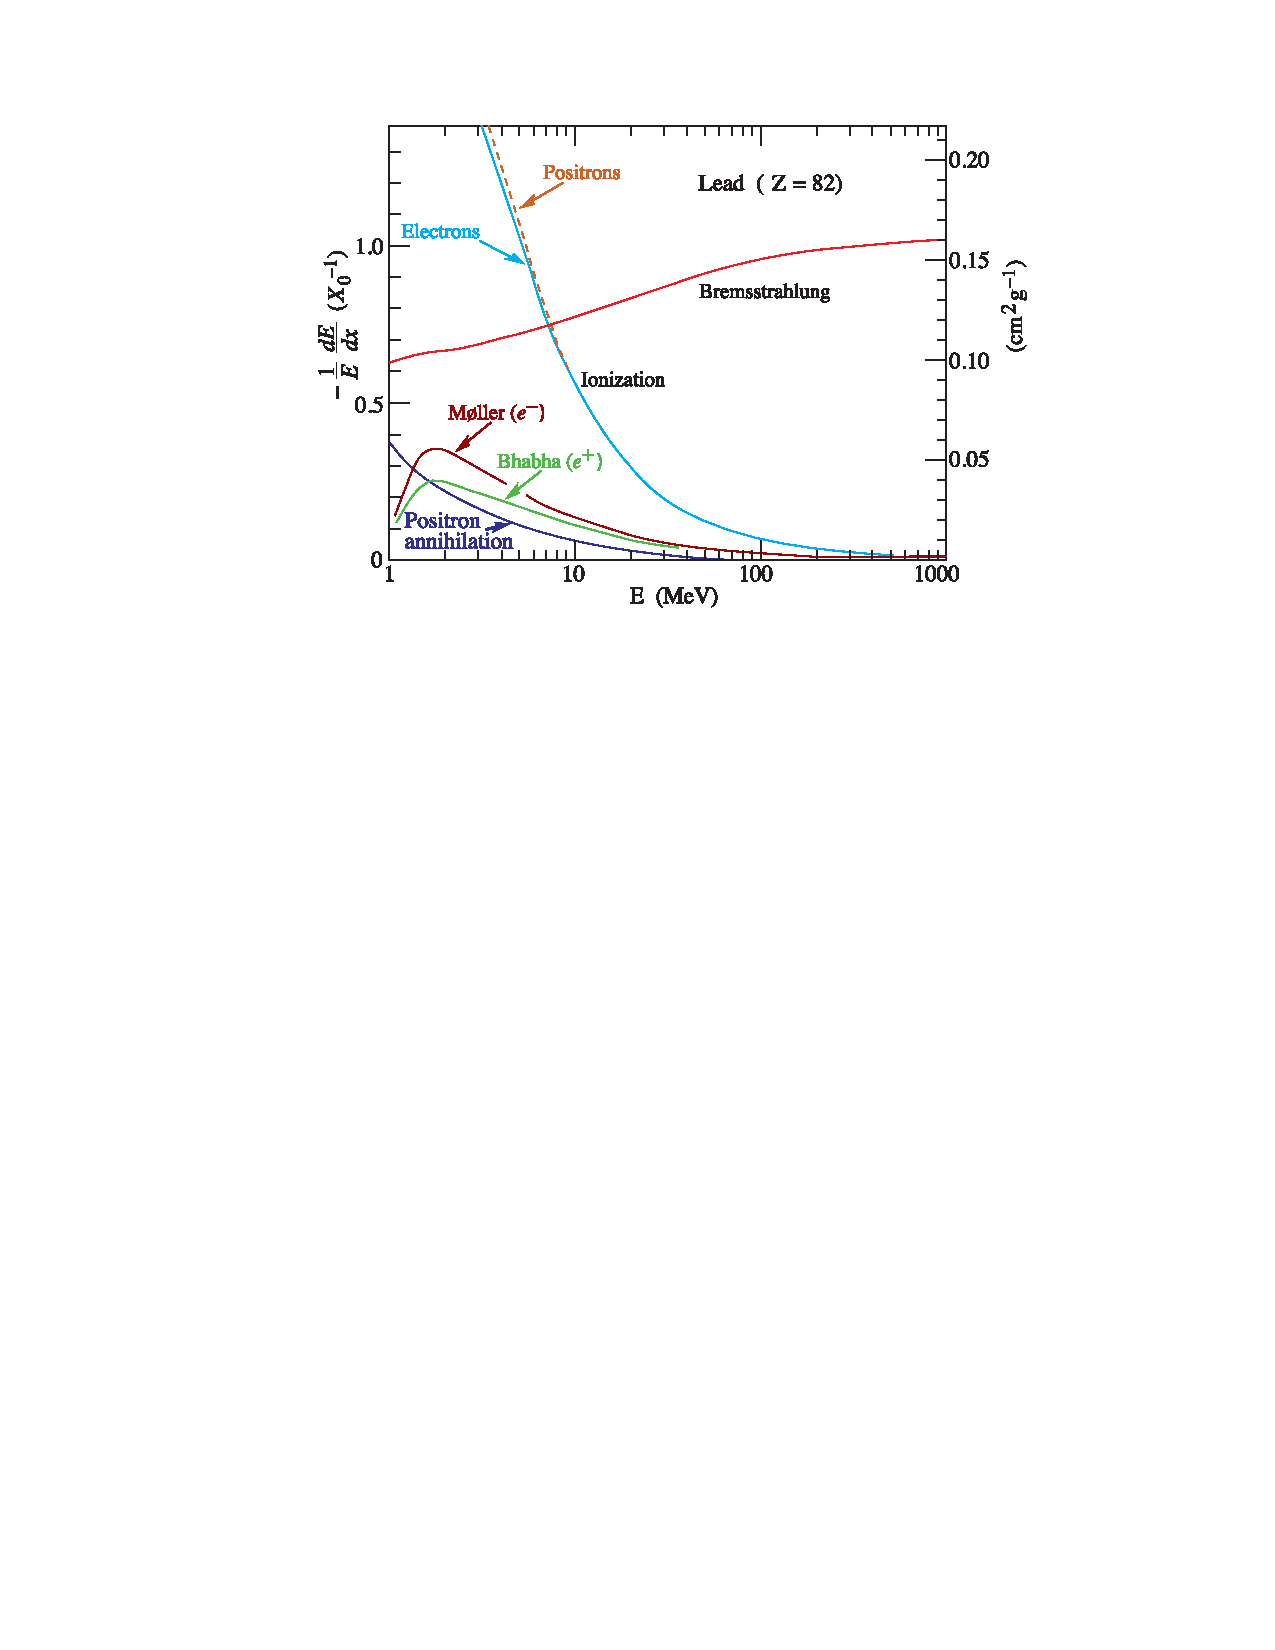
\includegraphics[width=0.58\textwidth]{figures/detector/electron_energy_loss}}
\subfigure[]{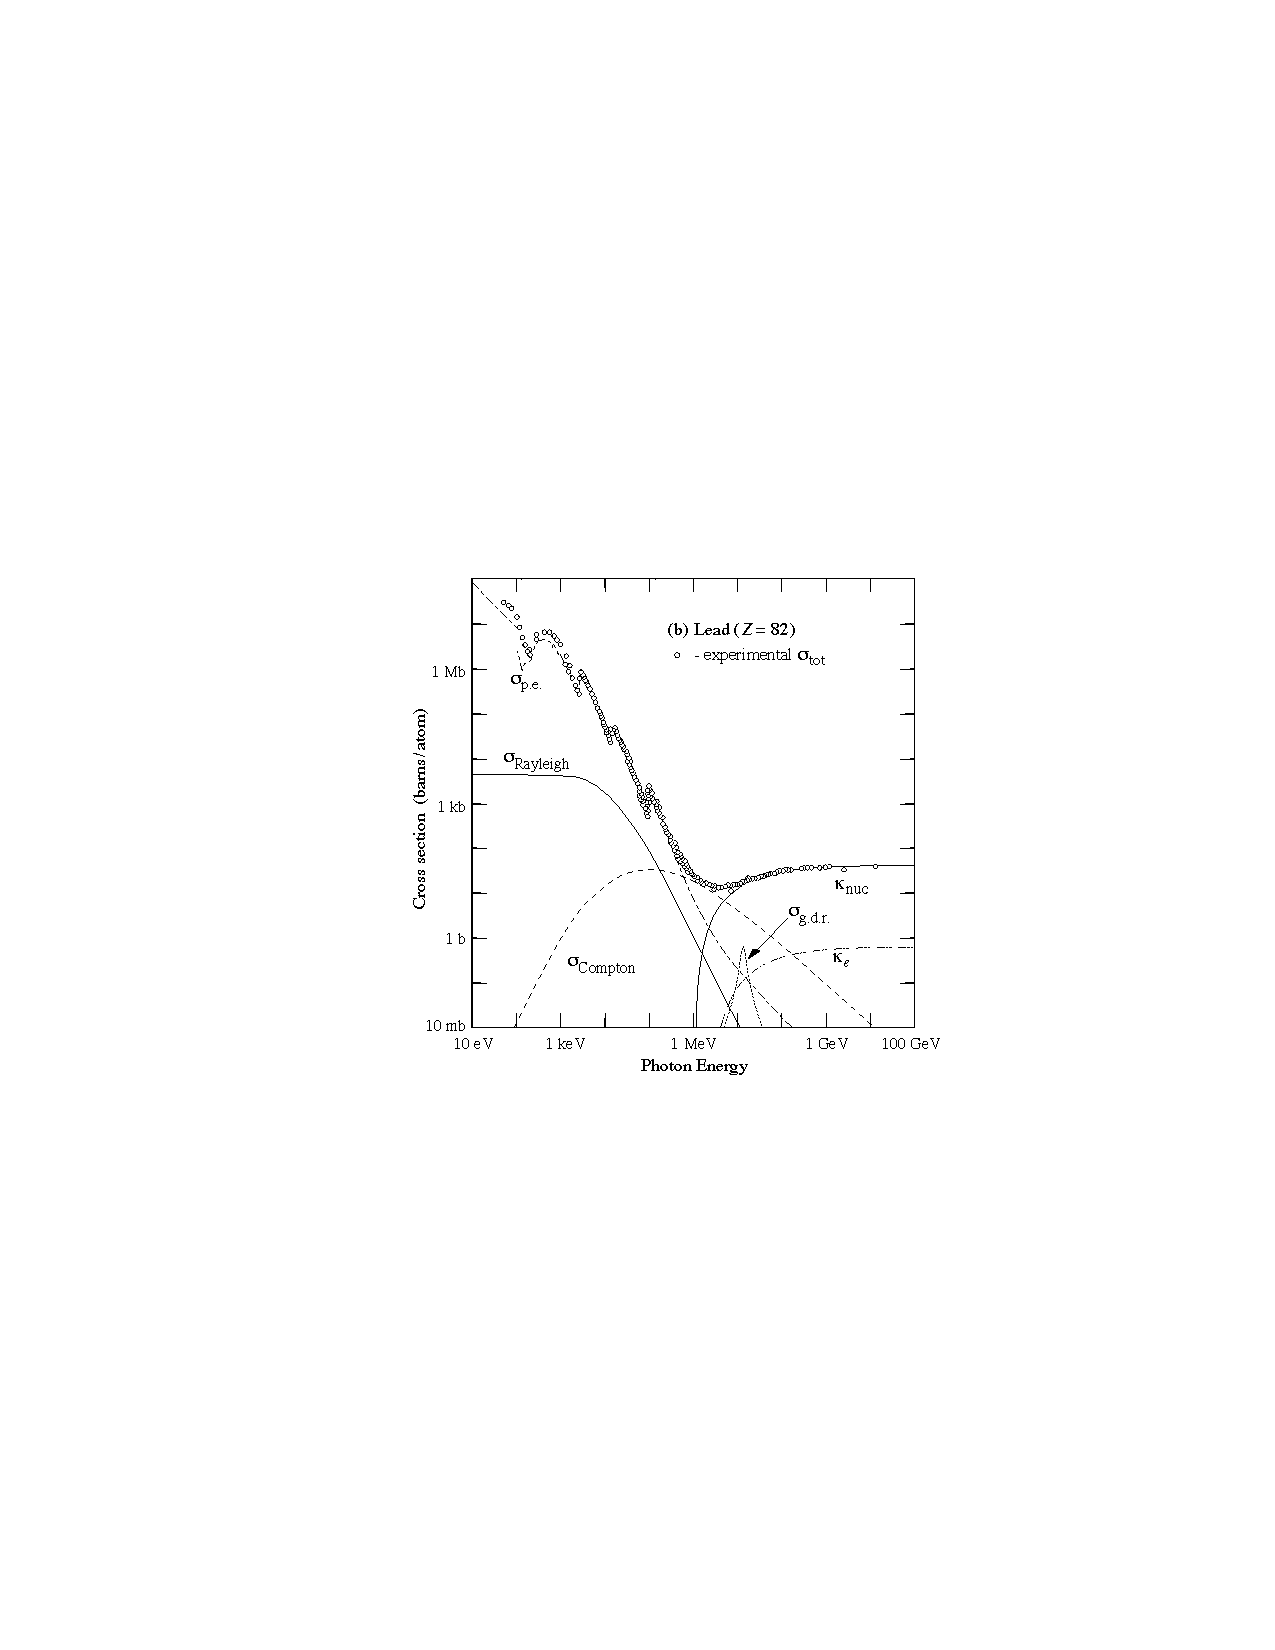
\includegraphics[width=0.4\textwidth]{figures/detector/photon_xsec}}
\caption{(a) Fractional energy loss per radiation length in lead as a function of the electron (positron) energy. (b) Photon interaction cross section in lead. Figures from Ref. \cite{Patrignani:2016xqp}. }
\label{fig:det:shower_elec}
\end{figure}


When electrons, positrons and photons with energies above 1 GeV traverse a block of material the produce a cascade of particles (\textit{electromagnetic shower}): electrons and positrons can emit a photon by Bremsstrahlung, and a photon (thanks to the interaction with a nucleus) can turn into an electron-positron pair (pair production is indicated with the symbol $\kappa_{nucl}$ in Fig. \ref{fig:det:shower_elec} (b)). A schematic view of the evolution of an electromagnetic shower is shown  in Fig. \ref{fig:det:shower_elec}(a). 

\begin{figure}[ht]
\centering
\subfigure[]{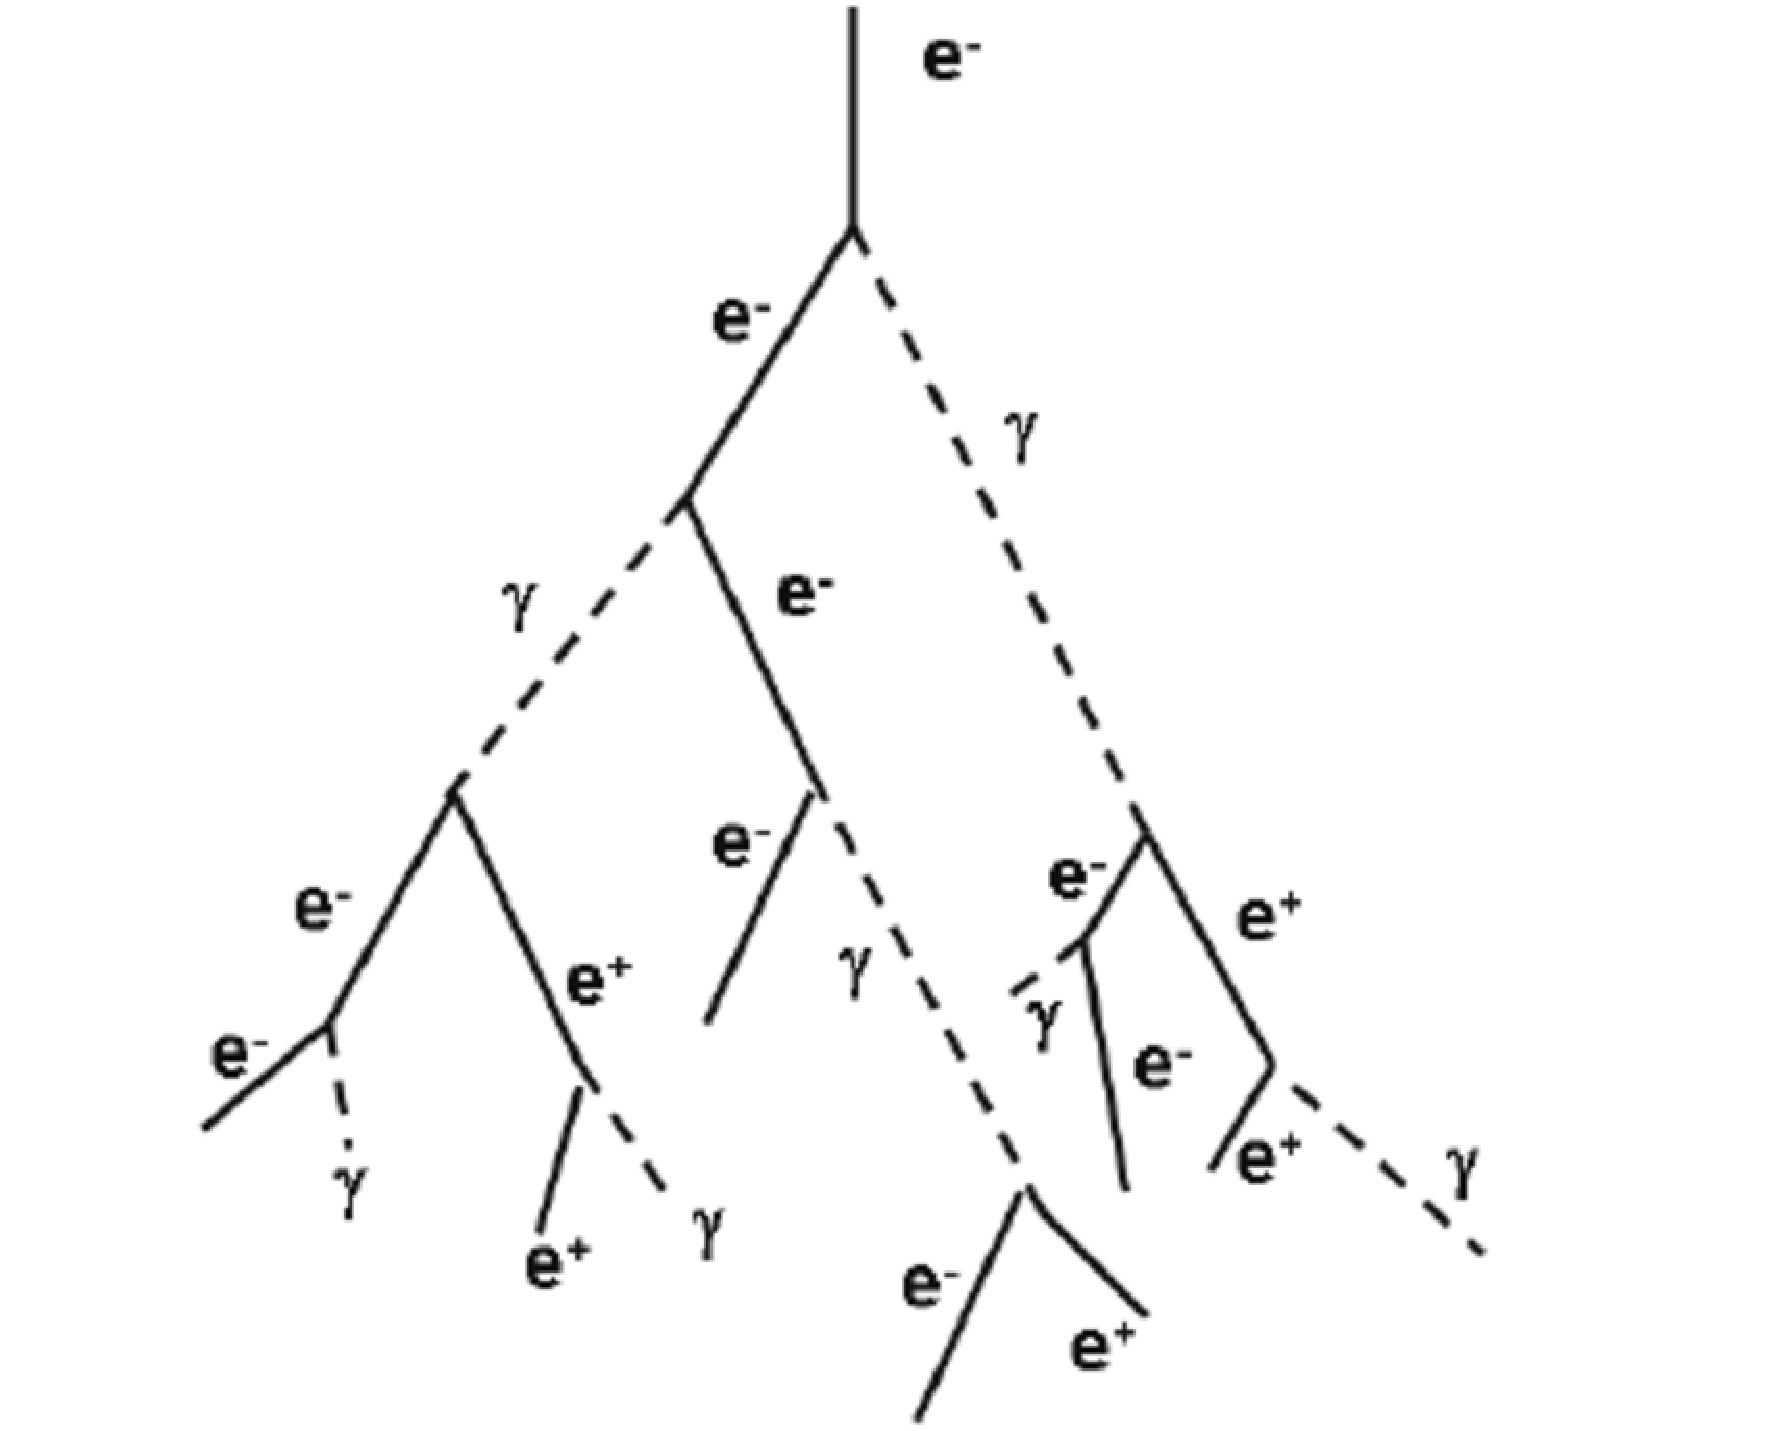
\includegraphics[width=0.45\textwidth]{figures/detector/elec_shower}}
\subfigure[]{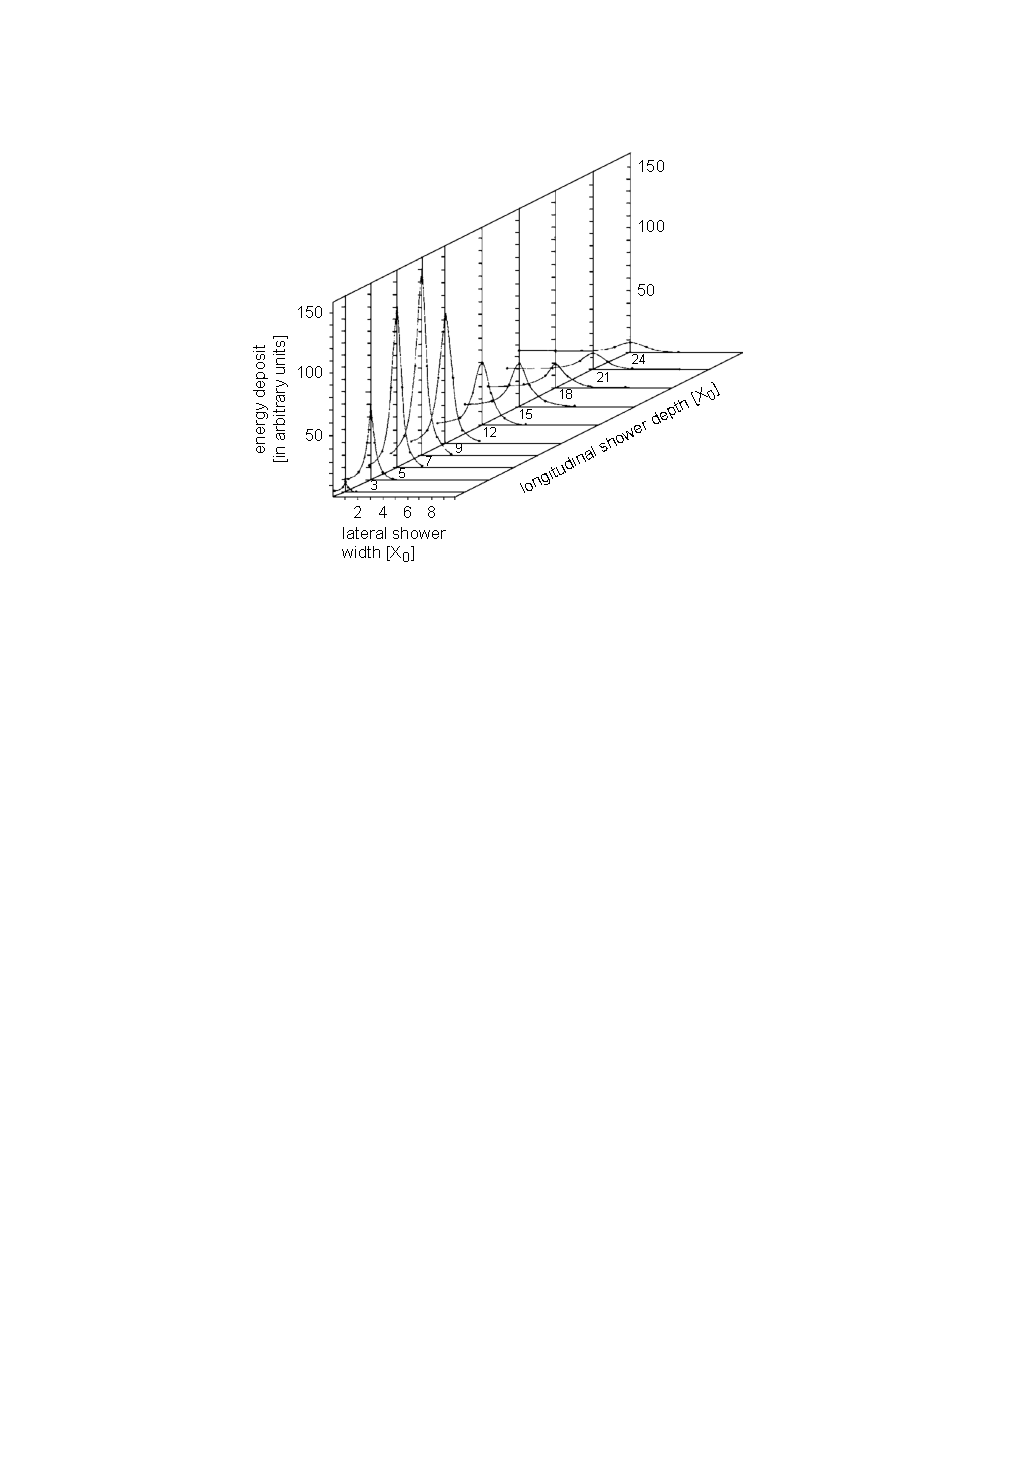
\includegraphics[width=0.52\textwidth]{figures/detector/elec_shower_lateral}}
\caption{(a) Sketch of the evolution of an electromagnetic shower. (b) Lateral and longitudianl evolution of the shower form 6-GeV electons. Figure from Ref. \cite{grupen_shwartz_2008}.}
\label{fig:det:shower_elec}
\end{figure}


The main parameter to describe the evolution of an electromagnetic shower is the \textit{radiation length} ($X_0$), defined as the distance over which an electron reduces its energy to $\frac{1}{e}$ of the initial value, and corresponds also to $\frac{7}{9}$ of the mean free path for pair production for a photon. The radiation length depends on the characteristics of the material:
\begin{equation}
X_0 [\frac{g}{cm^2}] = \frac{716 \frac{g}{ cm^2} A }{Z(Z+1) \ln\left(287/\sqrt{Z}\right)} \; ,
\end{equation}

where $A$ and $Z$ are the atomic and mass number of the material. If we define $t = \frac{x}{X_0}$ as the shower depth relative to the radiation length, the maximum number of produced particles occurs at:
\begin{equation}
t_{max} = \frac{\ln \left(E_0/E_c\right)}{ln\left(2\right)} \;.
\end{equation}
The typical values for the interaction length are of the order of the $cm$ (e.g. 0.56 cm for lead, 1.76 cm for iron \cite{Patrignani:2016xqp}); 99\% of the shower is contained in about 11(22) $X_0$ for a particle of 1 GeV(TeV), allowing for electromagnetic calorimeters of compact dimensions. 
The lateral with of the shower, determined mainly by multiple scattering, increases with depth and is defined in terms of the Moli\'ere radius:
\begin{equation}
R_M = \frac{21 MeV \; X_0[\frac{g}{cm^2}]}{E_c [MeV]} \; .
\end{equation}
A cylinder of radius 2$R_M$ contains about 95\% of the shower; for most calorimeters $R_M$ has a value of few centimeters, so electromagnetic showers are quite narrow. The longitudinal and lateral development of the shower induced in lead by 6-GeV electrons is shown in Fig. \ref{fig:det:shower_elec}(b).

Once the electrons in the shower have an energy lower than the \textit{critical energy} ($E_c$, defined as the energy where the loss through Bremsstrahlung equals the one through ionization), the shower stops as the energy is dissipated mostly through ionization for electrons and photoelectric effect for photons, and not anymore through the creation of new particles. Therefore all the energy of the incoming particle is in the end used to ionize the material of the detector, and this is the effect that is detected.


We have noticed in section \ref{sec:dec:tracking} how the resolution of the momentum measurement in a magnetic spectrometer decreases with the increase of the momentum itself. Instead, the relative energy resolution in a calorimeter improves for high-energy particles, and can be written in the parametric form:

\begin{equation}
\frac{\sigma_E}{E} = \sqrt{\left(\frac{a}{\sqrt{E}} \right)^2 + \left( \frac{b}{E} \right)^2 + c^2 } \; .
\end{equation}

The first term of the sum in quadrature reflects the \textit{stochastic} nature of the shower development: ignoring the instrumental effects, the energy resolution of a calorimeter is proportional to the square root of the total track length, which is in turn proportional to the initial energy. The contribution of this term is small in homogeneous calorimeters, while is larger in sampling calorimeters (because of fluctuations of the fraction of energy deposited in the absorber) and it grows with the thickness of the absorber layers; typical values for $a$ are 5-20\% if the energy is expressed in GeV. The second term is the \textit{noise term} coming from the electronic noise of the readout chain; this term is in general more relevant for calorimeters producing charge signals than for those producing light signals, and can become the dominant term for particles with energy below one GeV. The last term is a constant deriving from instrumental effects that produce a non-uniform detector response, including for example energy lost outside the detector volume and radiation damage; this becomes the dominant term at high energies and is typically $<1\%$. 



\subsubsection{Hadronic Calorimeters}

The difference between electromagnetic calorimeters and hadronic calorimeters finds its origin in the more complicated nature of strong interactions compared to the electromagnetic ones. 

A sketch of the evolution of an hadronic shower is shown in Fig. \ref{fig:det:shower_had}(a). A first relevant difference between hadronic and electromagnetic showers is that the former has a much larger spatial extension. On the longitudinal direction, the scale is determined by the \textit{nuclear interaction length} ($\lambda_I$), which is material-dependent and can be expressed as:
\begin{equation}
\lambda_I = 35 \frac{g}{cm^2} A^{1/3} \; ,
\end{equation}

where $A$ is the atomic number of the material. For most materials used in particle detectors this results to be larger than $X_0$ (e.g. the nuclear interaction length is 17.59 cm for lead, 16.77 cm for iron \cite{Patrignani:2016xqp}). The 99\% shower containment is reached after about 5(9) $\lambda_I$ for pions of 10(138) GeV. Also the lateral width of the sower results larger than in electromagnetic interactions: while the size of the Moli\'ere radius is determined mainly by multiple scattering, the lateral profile of an hadronic shower depends on the transverse-momentum transfer, that can be quite sizable in strong nuclear interactions. Fig. \ref{fig:det:shower_had}(b) shows the lateral shower profile for 10-GeV pions in iron.

\begin{figure}[ht]
\centering
\subfigure[]{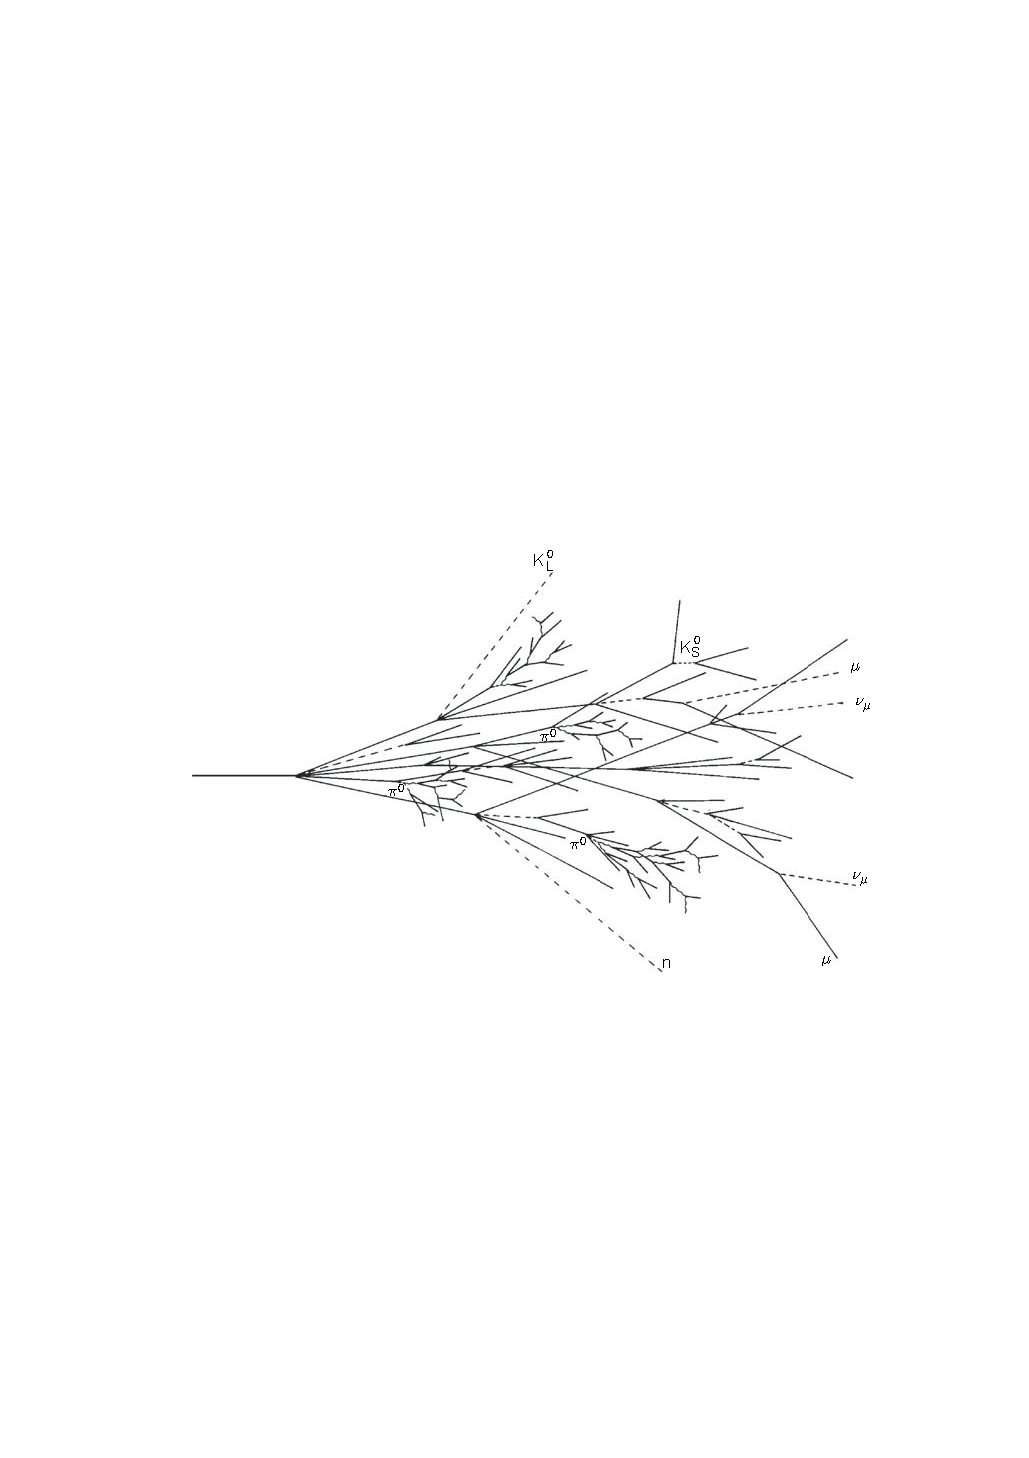
\includegraphics[width=0.48\textwidth]{figures/detector/hadron_shower}}
\subfigure[]{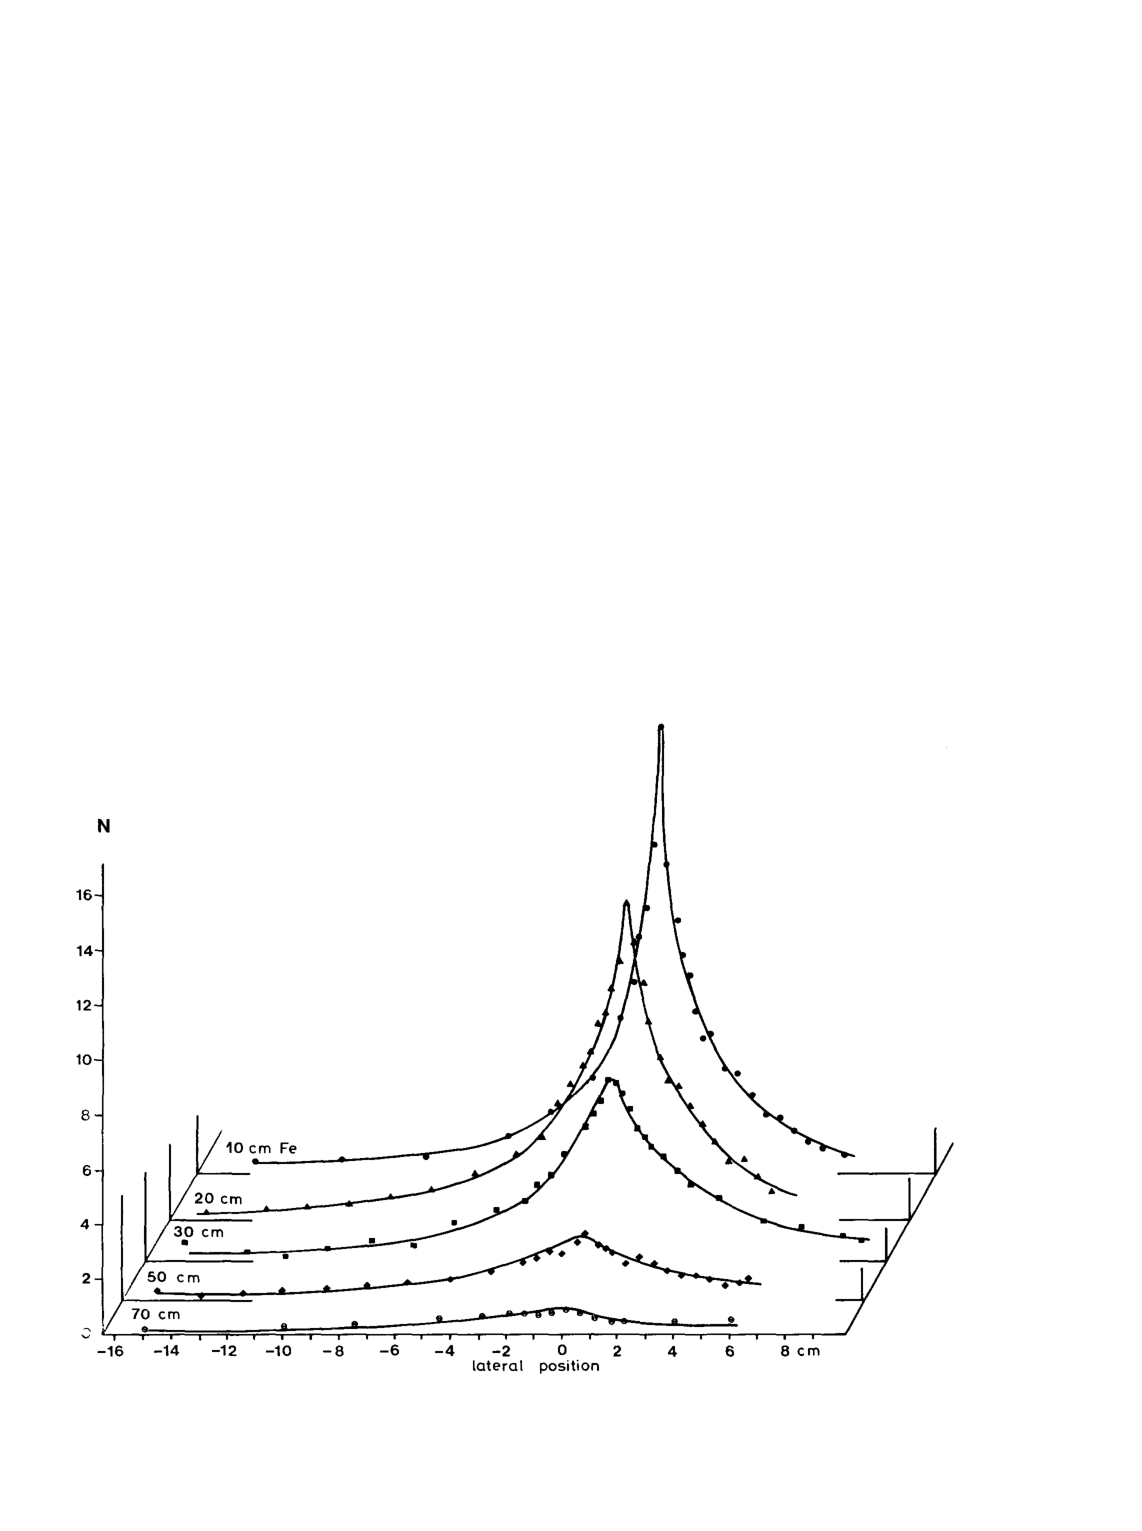
\includegraphics[width=0.48\textwidth]{figures/detector/hadron_shower_lateral}}
\caption{(a) Sketch of the evolution of an hadronic shower. Figure from Ref. \cite{grupen_shwartz_2008}. (b) Lateral energy distribution of shower induced by 10-GeV $\pi^-$, measured at a depth of 10, 20, 30, 50 and 70 cm in Fe. Figure from Ref. \cite{FRIEND1976505}.}
\label{fig:det:shower_had}
\end{figure}


% chiara: elaborate on the shower containment 

Another difference with electromagnetic showers lies in the composition of the shower: while an electromagnetic shower is constituted only by electrons, positrons and photons, a much larger variety of particles participates to hadronic showers, including both hadrons and electromagnetically-interacting particles. Starting from the simplifying assumption that one third of the particles produced in nuclear interactions are neutral pions ($f_{\pi^0}=\frac{1}{3}$), a first approximation of the electromagnetic fraction of a shower is given by:
\begin{equation}
f_{em} = 1 - \left(1 - \frac{1}{3} \right)^n \; ,
\end{equation}
where $n$ is the number of generations in the shower. Since the number of generations increases with the initial energy, it is intuitive that also $f_{em}$ will be larger for particles of higher energy. It is found \cite{GABRIEL1994336}:
\begin{equation}
f_{em} = 1 - \left(\frac{E}{E_0}\right)^{\left( k-1 \right)} \; ,
\end{equation}
where $E_0$ is the energy necessary to produce one pion (e.g. 0.7 GeV for iron and 1.3 GeV for lead), and $k$ is a slope parameter related to $f_{\pi^0}$ through the average multiplicity $<m>$:
\begin{equation}
1-f_{\pi^0} = <m>^{\left( k-1 \right)} \;.
\end{equation}


\begin{figure}[ht]
\centering
\subfigure{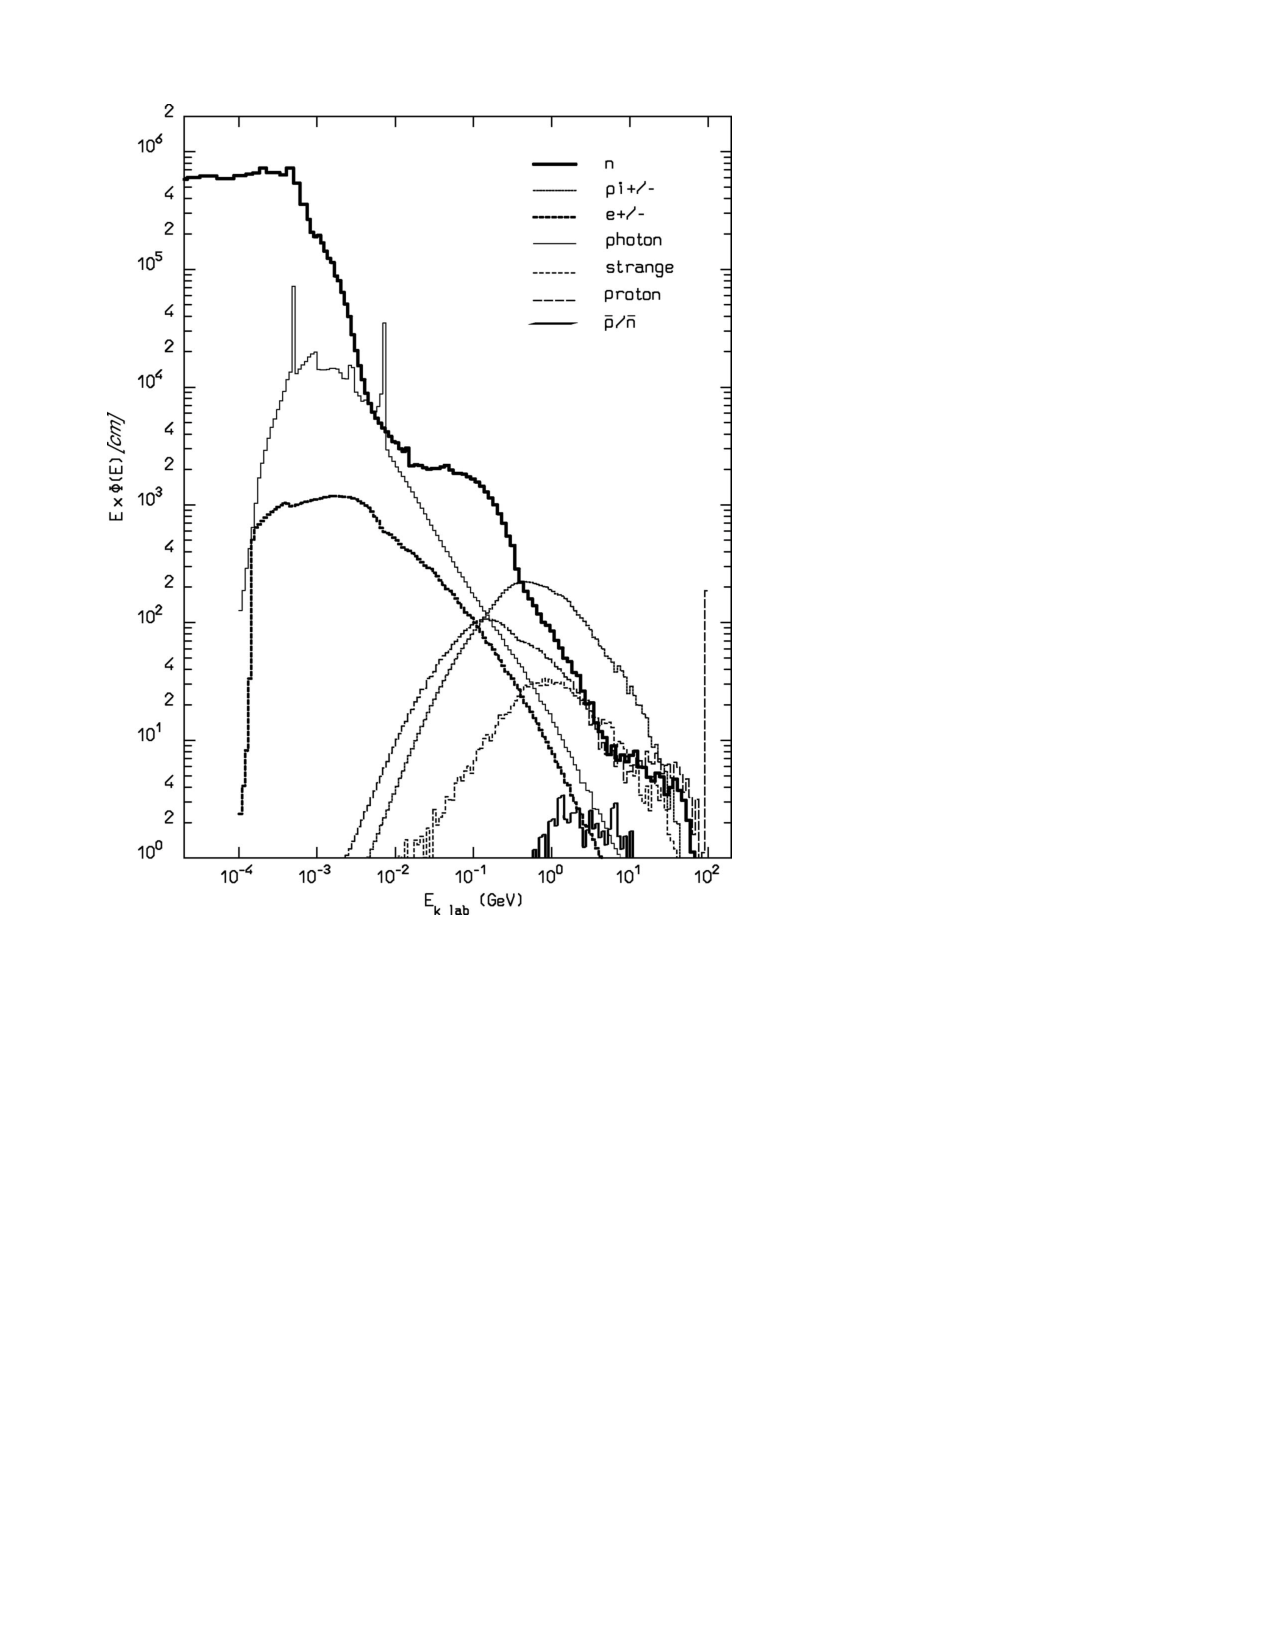
\includegraphics[width=0.42\textwidth]{figures/detector/had_shower_spectra}}
\caption{Particle spectra produced by 100-GeV protons absorbed by lead, as simulated by the Fluka code \cite{Ferrari:898301} and averaged over many showers.}
\label{fig:det:shower_had_spectra}
\end{figure}

Fig. \ref{fig:det:shower_had_spectra} shows the particle spectra produced by 100-GeV protons absorbed by lead, as simulated by the Fluka code \cite{Ferrari:898301}. We can see that at low energies the particle content is dominated by electrons, positrons, photons and neutrons.

While in electromagnetic showers most of the initial energy is recorded in the detector, in hadronic showers a relevant fraction (up to 30-40\%) is invisible. This invisible fraction is caused by energy that goes into breaking the nuclear bonds, nuclear fragments that in sampling calorimeters do not reach the active material, and neutral particles that can escape the calorimeter (e.g. neutrinos or long-lived neutral kaons). Therefore, for the same initial energy, the visible energy will be lower for an hadronic shower than for an electromagnetic one. If we define the \textit{response} as the collected signal per unit of incident energy, the invisible energy causes a different response of calorimeters to the electromagnetic and to the purely-hadronic parts of the shower. Defining $\eta_{em}$, $\eta_{h}$, $\eta_{\pi}$ respectively as the calorimeter response to electromagnetic shower, the hadronic part of the shower and to pions, we have that:
\begin{equation}
\eta_{\pi} = f_{em}\eta_{em} + (1-f_{em}) \eta_h = \eta_h \left( \frac{\eta_{em}}{\eta_{h}}f_{em} + (1-f_{em})  \right) \; .
\end{equation}

In general $\frac{\eta_{em}}{\eta_{h}}>1$. Since the value of the electromagnetic fraction is energy-dependent, the signal from the calorimeter does not increase linearly with energy. \textit{Compensating} calorimeters are the ones aiming at $\frac{\eta_{em}}{\eta_{h}}=1$, and to have the same response to the electromagnetic and hadronic part of the shower, restoring the linearity of the calorimeter response. In non-compensating calorimeters the fluctuations in $f_{em}$ are the dominant component of the energy resolution and, since the fluctuations are Gaussian, give rise to a term proportional to:

\begin{equation}
\frac{\sigma_E}{E} = \frac{\mathrm{const}}{\sqrt{E}}  \; .
\end{equation}
In modern non-compensating calorimeters the value of the constant is about 0.4, while it can be as low as 0.2 in the case of compensating calorimeters.




